\documentclass{article}
\usepackage[a4paper, total={6in, 8in}]{geometry}
\usepackage[utf8]{inputenc}

\title{Theoretical background}
\author{Dr. Siby Thomas}
\date{September, 2022}

\usepackage{natbib}
\usepackage{graphicx}

\begin{document}

\maketitle

\section{What problem are we trying to solve?}

We want to calculate the electronic structure of real materials, and their
physical properties by {\it{ab-initio}} method. Electrons are microscopic particle,
hence their dynamics is governed by the laws of quantum mechanics. Quantum
particles are described by the wave function.

$$
\lambda \cdot p = h
$$

where $h$ is the Plank constant. Wavefunction of an electron in a potential
filed $(V)$ is calculated by solving the Schrödinger equation:

$$
-\frac{\hbar^2}{2m} \nabla^2 \Psi(\textbf{r}, t) + V(\textbf{r}, t) = i\hbar
\frac{\partial\Psi(\textbf{r}, t)}{\partial t}
$$

Fortunately, in most practical purposes, the potential field is not a function
of time $(t)$, or even if it is a function of time, they changes relatively
slowly compared to the dynamics we are interested in. For example, the electrons
inside a material are subjected to the Coulomb filed of the nucleus. The nucleus
is heavy and their motion is much slower than the motion of the electrons. In
such situation, we can separate out the spacial and temporal parts of the wave
function:

$$
\Psi(\textbf{r}, t) = \psi(\textbf{r}) f(t)
$$

That reduces our task to solving only time independent Schrödinger equation:

$$
\left[-\frac{\hbar^2 \nabla^2}{2m} + v(\textbf{r})\right] \psi(\textbf{r}) =
\epsilon \psi(\textbf{r})
$$

Once we have the wavefunction, we can calculate the observables by taking the
expectation values.

$$
\braket{\psi_i | \psi_j} = \delta_{ij}
$$

$$
\braket{\psi_i | \hat{H} | \psi_i} = \epsilon_i
$$

However, the challenge is to solve the Schrödinger equation as a real physical
system is consists of large number of atoms. The Schrödinger equation becomes
coupled many-body equation.

$$\left[-\frac{\hbar}{2m} \sum_{i=1}^N \nabla_i^2 + \sum_{i=1}^NV(\textbf{r}_i)
+ \sum_{i=1}^N \sum_{j<i}U(\textbf{r}_i, \textbf{r}_j)\right]\psi(\textbf{r}_1,
\textbf{r}_2, ..., \textbf{r}_N)$$
$$= E\psi(\textbf{r}_1, \textbf{r}_2, ...,
\textbf{r}_N)$$

With today's available computing power, it is far from feasible to solve the
actual electronic wavefunction of a condensed matter system, where $N$ is of the
order of $10^{23}$.
%%%%%%%%%%%%%%%%%%%%%%%%%%%%%%%%%%%%%%%%%%%%%%%%%%%%%%%%%%%%%%%%%%%%%%%%%

\section{Hartree-Fock Theory}

Hatree-Fock theory is foundational to many electronic structure theory. It is an
independent particle model or mean filed theory. Consider we have two
non-interacting electrons. In that case, the Hamiltonian would be separable, and
the total wavefunction $\Psi(\textbf{r}_1, \textbf{r}_2)$ would be product of
the individual wave function. Now if we consider two electrons are forming a
single system, then there are two issues. (1) We can no longer ignore the
electron-electron interaction. (2) The wavefunction describing fermions must be
antisymmetric with respect to the interchange of any set of space-spin
coordinates. A simple **Hartree product** fails to satisfy that condition:

$$
\Psi_{HP}(\textbf{r}_1, \textbf{r}_2, \cdots, \textbf{r}_N) =
\phi_1(\textbf{r}_1) \phi_2(\textbf{r}_2) \cdots \phi_N(\textbf{r}_N)
$$

In oder to satisfy the antisymmetry condition, for our two electron system we
can formulate a total wavefunction of the form:

$$
\Psi(\textbf{r}_1, \textbf{r}_2) = \frac{1}{\sqrt{2}} [\chi_1(\textbf{r}_1)
\chi_2(\textbf{r}_2) - \chi_1(\textbf{r}_2)\chi_2(\textbf{r}_1)]
$$

## Slater determinant
The above equation can be written as:

$$
\Psi(\textbf{r}_1, \textbf{r}_2) = \frac{1}{\sqrt{2}}
\begin{vmatrix}
\chi_1(\textbf{r}_1) & \chi_2(\textbf{r}_1) \\
\chi_1(\textbf{r}_2) & \chi_2(\textbf{r}_2)
\end{vmatrix}
$$

Now what happens if we have more than two electrons? We can generalize the above
determinant form to $N$ electrons:

$$
\Psi = \frac{1}{\sqrt{N!}}
\begin{vmatrix}
\chi_1(\textbf{r}_1) & \chi_2(\textbf{r}_1) & \cdots & \chi_N(\textbf{r}_1) \\
\chi_1(\textbf{r}_2) & \chi_2(\textbf{r}_2) & \cdots & \chi_N(\textbf{r}_2) \\
\vdots & \vdots & \ddots & \vdots \\
\chi_1(\textbf{r}_N) & \chi_2(\textbf{r}_N) & \cdots & \chi_N(\textbf{r}_N)
\end{vmatrix}
$$

The above antisymmetrized product can describe electrons that move independently
of each other while they experience an average (mean-field) Coulomb force.\\

## Resources
- <http://vergil.chemistry.gatech.edu/notes/hf-intro/hf-intro.html>

%%%%%%%%%%%%%%%%%%%%%%%%%%%%%%%%%%%%%%%%%%%%%%%%%%

\section{Introduction to Density Functional Theory}

Density functional theory (DFT) approaches the many-body problem by focusing on
the electronic density which a function of three spacial coordinates instead of
finding the  wave functions. DFT tries to minimize the energy of a system
(ground state) in a self consistent way, and it is very successful in
calculating the electronic structure of solid state systems.\\

:::info

A functional is a function whose argument is itself a function. $f(x)$ is a
function of the variable $x$ while $F[f]$ is a functional of the function $f$.

$$
y = f(x)
$$

$f$ is a function, it takes a number $x$ as input and output $y$ is also a
number.

$$
y = F[f(x)]
$$

$F$ is a functional it takes function $f(x)$ as input and output $y$ is a
number.

:::\\

\subsection{Hohenberg-Kohn Theorem 1}
The ground state density $$n(\textbf{r})$$ determines the external potential
energy $$v(\textbf{r})$$ to within a trivial additive constant.

So what Hohenberg-Kohn theorem says, may not sound very trivial. Schrödinger
equation says how we can get the wavefunction from a given potential. Then there
is the Schrödinger equation, if we can solve it (which could be difficult), we
know how to get the density. Now Hohenberg and Kohn says the opposite is also
true. For a given density, the potential can be uniquely determined. For
non-degenerate ground states, two different Hamiltonian cannot have the same
ground-state electron density. It is possible to define the ground-state energy
as a function of electronic density.\\

\subsection{Hohenberg-Kohn Theorem 2}
Total energy of the system $E(n)$ is minimal when $n(\textbf{r})$ is the
actual ground-state density, among all possible electron densities.

The ground state energy can therefore be found by minimizing $E(n)$ instead of
solving for the many-electron wavefunction. However, note that HK theorems do
not tell us how the energy depends on the electron density. In reality, apart
form some special cases, the exact $E(n)$ is unknown and only approximate
functionals are used.\\

\subsection{Kohn-Sham hypothesis}
 For any system of $N$ interacting electrons in a given external potential
$v_{ext} (\textbf{r})$, there is a virtual system of $N$ non-interacting
electrons with exactly the same density as the interacting one. The
non-interacting electrons subjected to a different external (single particle)
potential.

$$
\left[-\frac{\hbar^2 \nabla^2}{2m} + v_s(\textbf{r}) \right] \psi_i(\textbf{r})
= \epsilon_i \psi_i(\textbf{r})
$$

$$
v_s(\textbf{r}) = v_{ext}(\textbf{r}) + e^2 \int d^3r'
\frac{n(\textbf{r})}{|\textbf{r} - \textbf{r}'|} + v_{xc}(\textbf{r}; [n])
$$

$$
n(\textbf{r}) = \sum_i f_i |\psi_i (\textbf{r})|^2
$$

where $f_i$ is the occupation factor of electrons ($0 \le f_i \le 2$). The
KS equation looks like single particle Schrödinger equation, however $e^2 \int
d^3r' \frac{n(\textbf{r})}{|\textbf{r} - \textbf{r}'|}$ and $v_{xc} (\textbf{r};
[n])$ terms depend on $n(\textbf{r})$ i.e., on $\psi_i$ which in turn depends on
$v_{ext}$. Therefore the problem is non-linear. It is usually solved
computationally by starting from a trial potential and iterate to
self-consistency. Also note that we have not included the kinetic energy term
for the nucleus. This is because the nuclear mass is about three orders of
magnitude heavier than the electronic mass ($M \gg m)$, so essentially
electronic dynamics is much faster than the nuclear dynamics (see
Born-Oppenheimer approximation).\\


:::info

$v_{ext}(\textbf{r})$ includes the potential energy due to nuclear field, and
external electric and magnetic fields if present.

:::\\


\subsection{Algorithmic implementation}
We can write our Schrödinger in Dirac Bra-Ket notation:

$$
\hat{H} \ket{\psi} = E\ket{\psi}
$$

We start with an initial guess for the electron density $n(\textbf{r})$, and
construct a pseudo potential for the nuclear potential. In tern, we have the
Hamiltonian. Solve for $\psi_i(\textbf{r})$, subsequently $n(\textbf{r})$, and
iterate until self consistency is achieved.\\

\begin{figure}[h!]
\centering
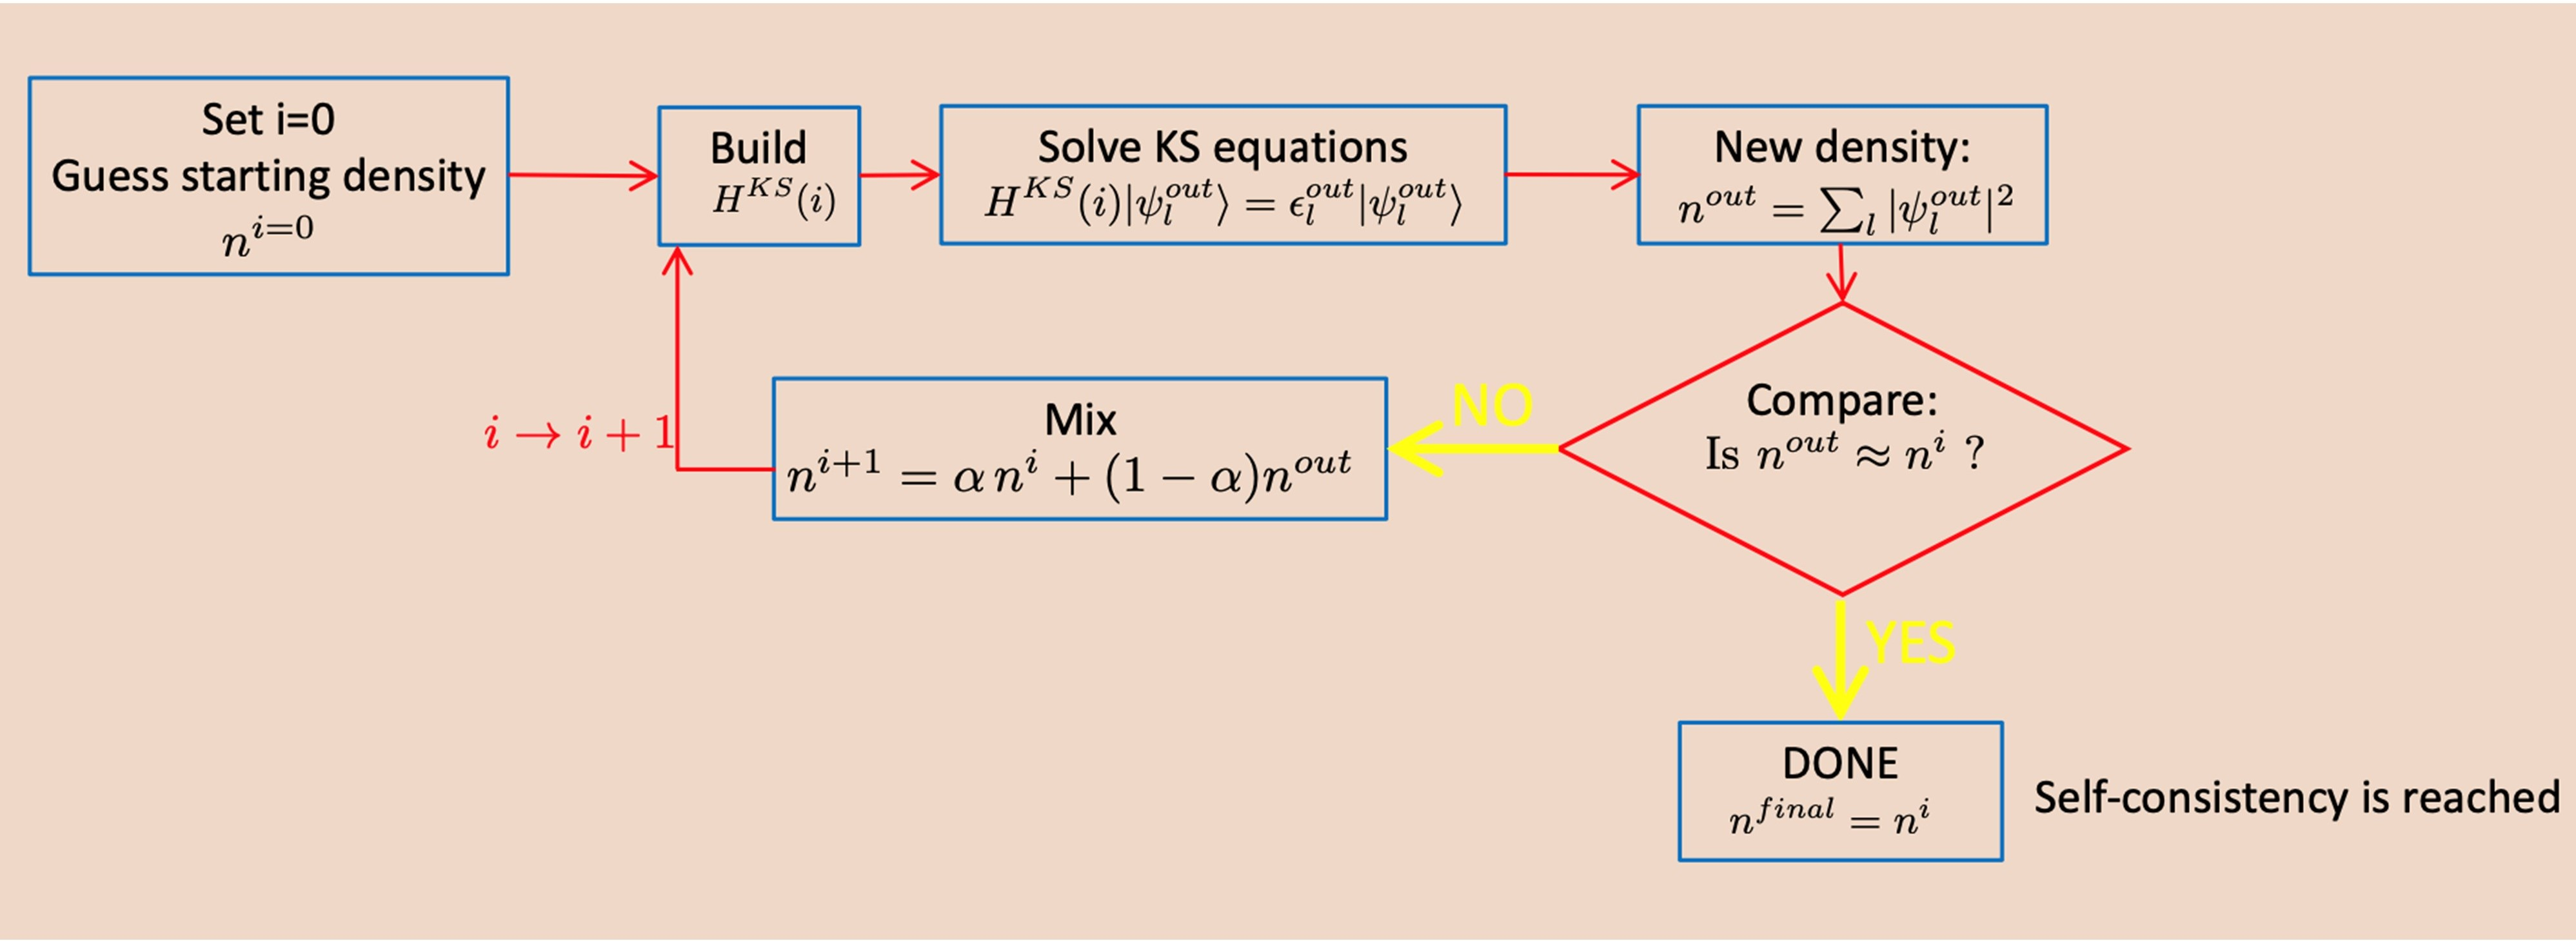
\includegraphics[scale=0.4]{SCF.jpg}
\caption{Self consistency loop in DFT calculation. The above screenshot was taken from lecture slide of Professor Ralph Gevauer from  ICTP MAX School 2021.}
\label{fig:univerise}
\end{figure}

\\
The potential due to the ions is replaced by the pseudo potentials which removes
the oscillations near the atomic core (reducing number of required plane wave
basis vectors) and simulates the exact behavior elsewhere. The pseudo potential
is also different for different exchange correlation functional, and it is
specified in the pseudo potential file. If a system had more than one type of
atom, always choose the pseudo potentials with same exchange correlation (e.g.,
PBE).\\

It is important to note that DFT is calculations are not exact solution to the
real systems because exact functional ($v_{xc}$) we need to solve the Kohn-Sham
equation is not known. Therefore, we have to compare the results with
experimental observations.

\subsection{Plane-wave expansion}

The wavefunctions are expanded in terms of a basis set. In quantum espresso, the
the basis function is plane waves. There exists other DFT codes that uses
localized basis function as well. Plane waves are simpler but generally requires
much large number of them compared to other localized basis sets.\\

$$
\psi_i(\textbf{r}) = \sum_{\alpha = 1} ^{N_b} c_{i\alpha} f_{\alpha}(\textbf{r})
$$

Where $N_b$ is the size basis set. Then the eigenvalue equation becomes:

$$
\sum_{\beta} \rm{H}_{\alpha\beta} c_{i\beta} = \epsilon_i c_{i\alpha}
$$

$$
\Rightarrow
\begin{pmatrix}
H_{11} &  ... & H_{1b} \\
... & ... & ... \\
H_{b1} & ... & H_{bb}
\end{pmatrix}
\begin{pmatrix}
c_1 \\
... \\
c_b
\end{pmatrix}
= \epsilon_i
\begin{pmatrix}
c_1 \\
... \\
c_b
\end{pmatrix}
$$

This is a linear algebra problem, solving the above involves diagonalization of
($N_b \times N_b$) matrix which gives us corresponding eigenvalue and
eigenfunction.\\

\subsection{Variational Principle}
Finding the ground state:

$$
E[\Phi] = \frac{\braket{\Phi | \hat H | \Phi}}{\braket{\Phi|\Phi}}
$$

$$
E[\Phi] \ge E_0
$$

## Bloch theorem

$$
\psi_k(r) = e^{i \textbf{k} \cdot \textbf{r}} u_k(\textbf{r})
$$

$$
u_k(\textbf{r}) = u_k(\textbf{r} + \textbf{R})
$$

$$\textbf{R}$$ is lattice vector.

Fourier expansion:

$$
u_k(\textbf{r}) = \frac{1}{\Omega} \sum_G c_{\textbf{k,G}} e^{i \textbf{G} \cdot
\textbf{r}}
$$

$$\textbf{G}$$ is reciprocal lattice vector.

$$
\psi_k(\textbf{r}) = \frac{1}{\Omega} \sum_G c_{\textbf{k,G}}
e^{i (\textbf{k + G}) \cdot \textbf{r}}
$$

Contribution from higher Fourier components are small, we can limit the sum at
finite $|\textbf{k + G}|$

$$
\frac{\hbar^2 |\textbf{k + G}|}{2m} \le E_{cutoff}
$$

The charge density can be obtained from:

$$
n(\textbf{r}) = \sum_k \psi_k^*(\textbf{r}) \psi_k(\textbf{r})
$$

We need two set of basis vectors: one to store the wavefunctions, and another
for the charge density.\\

:::info

We need about 4 times the cutoff for the charge density compared to the cutoff
for the wavefunction. In case of ultrasoft pseudo potentials, we require lower
cutoff for energy, therefore `ecutrho` might require 8 or 12 times higher than
the `ecutwfc`.\\

:::\\

\subsection{Resources}

\item{[MIT Course](https://ocw.mit.edu/courses/materials-science-and-engineering/3-320-atomistic-computer-modeling-of-materials-sma-5107-spring-2005/video-lectures/)}
\item {[Quantum Espresso Tutorials](https://www.quantum-espresso.org/resources/tutorials)}
\item{[http://compmatphys.epotentia.com](http://compmatphys.epotentia.com/)}


%%%%%%%%%%%%%%%%%%%%%%%%%%%%%%%%%%%%%%%%%%%%%%%%%%
\section{Pseudo potentials}
In Quantum Espresso, pseudopotential replaces the actual electron-ion
interaction. The pseudopotential describes the atomic nucleus and all the
electrons except teh outermost valence shell. The the rapidly changing potential
field near the atomic core is replaced by a smoother function that simulates the
potential field far from the core very well. By doing so, it requires less
number plane wave basis for wavefunction expansion.\\

We can choose form various pseudopotential libraries. Choice of pseudopotential
depends on the problem we are investigating, e.g., if there is a heavy element
present in our system and we are interested in the spin-orbit coupling effects,
we should choose a full relativistic pseudo potential. We need to be careful
whether our chosen pseudo potential correctly reproduces physical properties.
Various pseudopotential libraries:\\

\item{https://www.quantum-espresso.org/pseudopotentials (https://www.quantum-espresso.org/pseudopotentials)}
\item{https://www.materialscloud.org/discover/sssp/table/efficiency\\
(https://www.materialscloud.org/discover/sssp/table/efficiency)}\\
\item {http://www.pseudo-dojo.org (http://www.pseudo-dojo.org)}\\
\item{https://www.physics.rutgers.edu/gbrv/ (https://www.physics.rutgers.edu/gbrv/)}\\

Ultra soft pseudo potentials are computationally efficient than the norm
conserving pseudo potentials. You will find the recommended `ecutwfc` in the
header of each pseudo potential file. If you choose an ultra-soft pseudo
potential, you will need `ecutrho` about 8 times the value of `ecutwfc`. The
default `ecutrho` is 4 times `ecutwfc` in Quantum Espresso code, which is a
good choice for norm conserving pseudo potentials. You should check energy
convergence against `ecutwfc` for your system.\\

By using pseudo potential, we want to get rid of the core electrons that do not
participate in the chemical properties of material. This is known also as rigid
core approximation. Instead of accounting the nucleus and core electrons
separately, we want to have a pseudo potential that interacts in a similar way
with the valence electrons.\\

:::info

\item We can mix different types of pseudo potentials (e.g., norm conserving,
ultra-soft, or PAW), but we cannot mix different functional (e.g., PBE and LDA).\\

\item "sol" in PBE-sol stands for solid. For bulk systems PBE-sol should be used,
while PBE is appropriate for molecules. In case of 2D materials generally PBE is
chosen, but one can check PBE-sol.\\

:::

:::danger Common error

If you mix PBE with PBE-sol type, it results in Error: conflicting values for
igcx. However, it is allowed to mix those two types of pseudo. We can set
desired exchange functional via input$_$dft instead of reading from the pseudo
potential file.

:::\\

\subsection{Resources}
\item{Naming convention for PP files (https://www.quantum-espresso.org/pseudopotentials/naming-convention)}













%\begin{figure}[h!]
%\centering
%\includegraphics[scale=1.7]{universe.jpg}
%\caption{The Universe}
%\label{fig:univerise}
%\end{figure}

%\section{Conclusion}
%``I always thought something was fundamentally wrong with the universe'' \citep{adams1995hitchhiker}

%\bibliographystyle{plain}
%\bibliography{references}
\end{document}
